\tikzset{every picture/.style={line width=0.75pt}} %set default line width to 0.75pt        

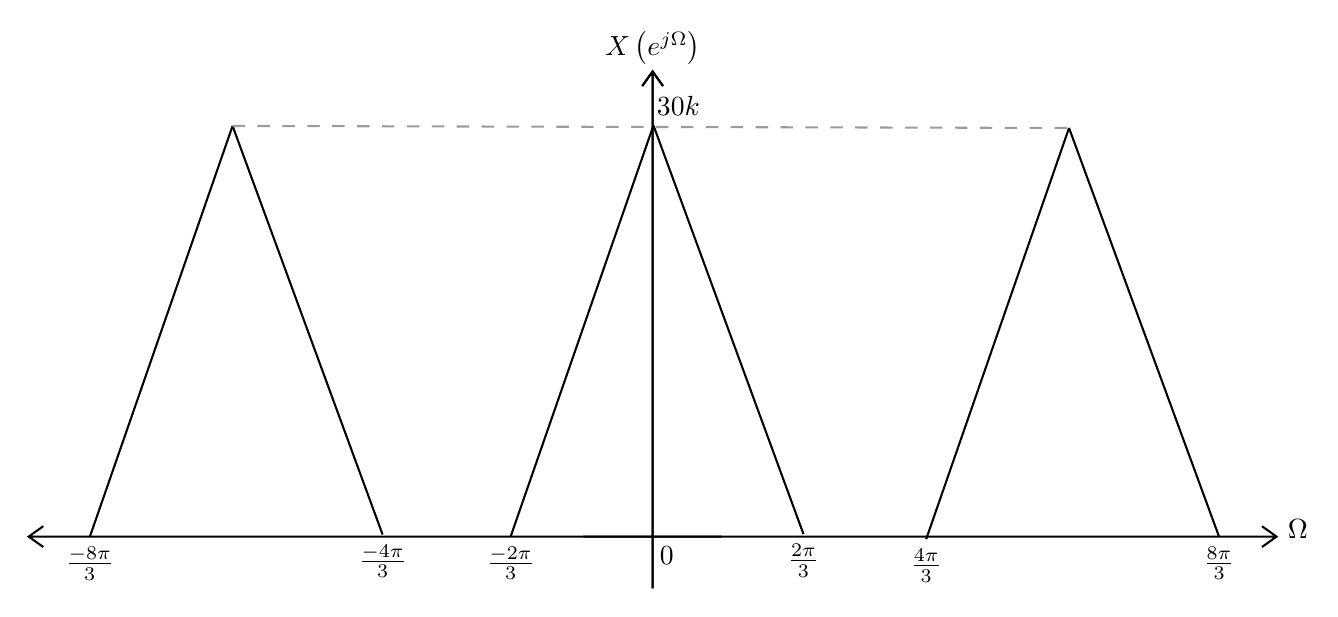
\begin{tikzpicture}[x=0.75pt,y=0.75pt,yscale=-1,xscale=1]
%uncomment if require: \path (0,393); %set diagram left start at 0, and has height of 393

%Shape: Axis 2D [id:dp1655481678492966] 
\draw  (281,257.1) -- (615,257.1)(314.4,33) -- (314.4,282) (608,252.1) -- (615,257.1) -- (608,262.1) (309.4,40) -- (314.4,33) -- (319.4,40)  ;
%Shape: Axis 2D [id:dp38625059588045074] 
\draw  (347.8,257.1) -- (13.8,257.1)(314.4,33) -- (314.4,282) (20.8,252.1) -- (13.8,257.1) -- (20.8,262.1) (319.4,40) -- (314.4,33) -- (309.4,40)  ;
%Straight Lines [id:da9294018403143072] 
\draw    (245.98,257.1) -- (314.8,59) ;
%Straight Lines [id:da9740337393831212] 
\draw    (387.07,255.87) -- (314.8,59) ;
%Straight Lines [id:da9384743114749254] 
\draw    (587.29,257.1) -- (515.02,60.23) ;
%Straight Lines [id:da5891124578320841] 
\draw    (446.2,258.33) -- (515.02,60.23) ;
%Straight Lines [id:da1820199963240804] 
\draw    (184.29,256.1) -- (112.02,59.23) ;
%Straight Lines [id:da7845075875180415] 
\draw    (43.2,257.33) -- (112.02,59.23) ;
%Straight Lines [id:da45856677787947864] 
\draw [color={rgb, 255:red, 155; green, 155; blue, 155 }  ,draw opacity=1 ] [dash pattern={on 4.5pt off 4.5pt}]  (112.02,59.23) -- (515.02,60.23) ;

% Text Node
\draw (619,247.4) node [anchor=north west][inner sep=0.75pt]    {$\Omega $};
% Text Node
\draw (290,12.4) node [anchor=north west][inner sep=0.75pt]    {$X\left( e^{j\Omega }\right)$};
% Text Node
\draw (316.4,260.5) node [anchor=north west][inner sep=0.75pt]    {$0$};
% Text Node
\draw (587.29,260.5) node [anchor=north] [inner sep=0.75pt]    {$\frac{8\pi }{3}$};
% Text Node
\draw (315,43.4) node [anchor=north west][inner sep=0.75pt]    {$30k$};
% Text Node
\draw (446.2,261.73) node [anchor=north] [inner sep=0.75pt]    {$\frac{4\pi }{3}$};
% Text Node
\draw (387.07,259.27) node [anchor=north] [inner sep=0.75pt]    {$\frac{2\pi }{3}$};
% Text Node
\draw (245.98,260.5) node [anchor=north] [inner sep=0.75pt]    {$\frac{-2\pi }{3}$};
% Text Node
\draw (184.29,259.5) node [anchor=north] [inner sep=0.75pt]    {$\frac{-4\pi }{3}$};
% Text Node
\draw (43.2,260.73) node [anchor=north] [inner sep=0.75pt]    {$\frac{-8\pi }{3}$};


\end{tikzpicture}
